\graphicspath{{solutionImages/}}
\chapter{Implémentation d’un agent conversationnel}

Le dernier chapitre nous a permis d’identifier diverses méthodes existantes. En fonction des besoins que nous avons mis en avant, nous avons pu retenir celle des intents. Cette méthode consiste à choisir le bon intent par rapport à la phrase d’un utilisateur pour fournir la meilleure réponse possible. L’intent permettra aussi à une application de déclencher un processus de dialogue pour répondre à une tâche possible du chatbot en utilisant tous les services externes disponibles pour ajouter de l’intelligence dans la réflexion.

\section{Méthodologie}

Pour étudier le paramétrage d’un chatbot avec la méthode choisie, nous utiliserons LUIS pour gérer le langage naturel couplé avec Microsoft bot framework pour programmer. Un scénario réel d’un chatbot effectuant un service sera développé et nous allons montrer quelles ont été les réflexions dans la phase de création par rapport à la compréhension du langage.

\subsection{Microsoft bot framework}

Microsoft bot framework est une architecture pour créer des chatbots, les connecter sur des canaux de discussions, les tester sur un émulateur, et les déployer sur les plateformes botframework pour les rendre accessibles et azure pour offrir davantage de services liés au machine learning ou à l’analytics.
\vspace{1em}

Le développement se fera en C\# sous Visual Studio 2015 et l’exécution du chatbot et les tests seront faits avec Bot Framework Channel Emulator.

\subsection{LUIS}

LUIS est un service de Microsoft Azure pour comprendre le langage naturel. Il gère les intents comme expliqué dans la partie état de l’art.
\vspace{1em}

Diagramme de LUIS : 

\begin{figure}[H]
	\centering
		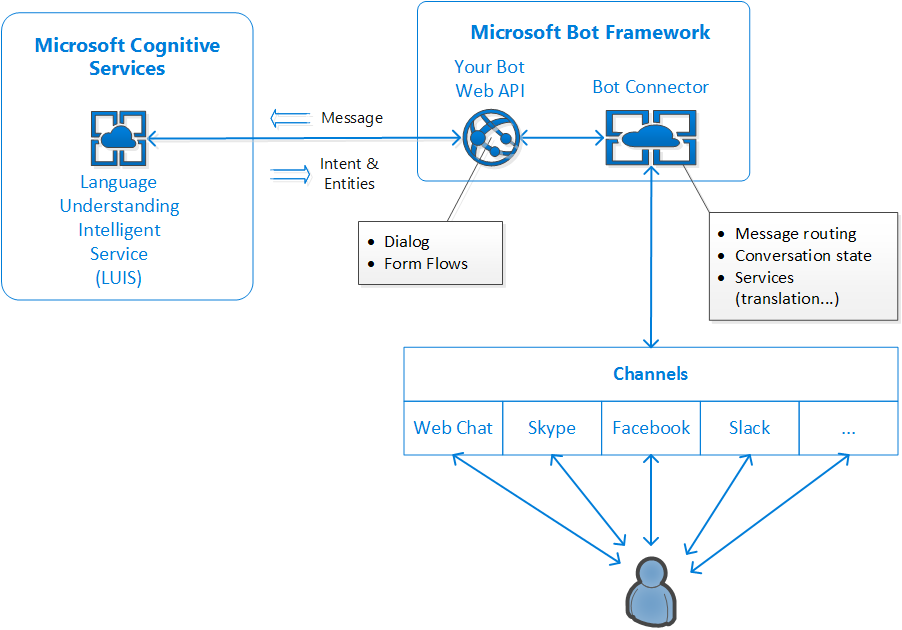
\includegraphics[width = 0.8\textwidth]{LUIS.png}
	\caption{LUIS architecture}
	\label{fig:LUIS architecture}
\end{figure}

Il y a deux autres services utiles, mais non utilisés dans ma solution qui seraient pourtant très utiles dans la phase de compréhension en amont de celle avant l’utilisation de LUIS :
\vspace{1em}

- API vérification orthographique Bing : pour une correction orthographique avec un renvoi de meilleurs résultats.
\vspace{1em}

Exemple : Je voudari commander une piza donne : je voudrais commander une pizza.
Le résultat en JSON :

\begin{figure}[H]
	\centering
		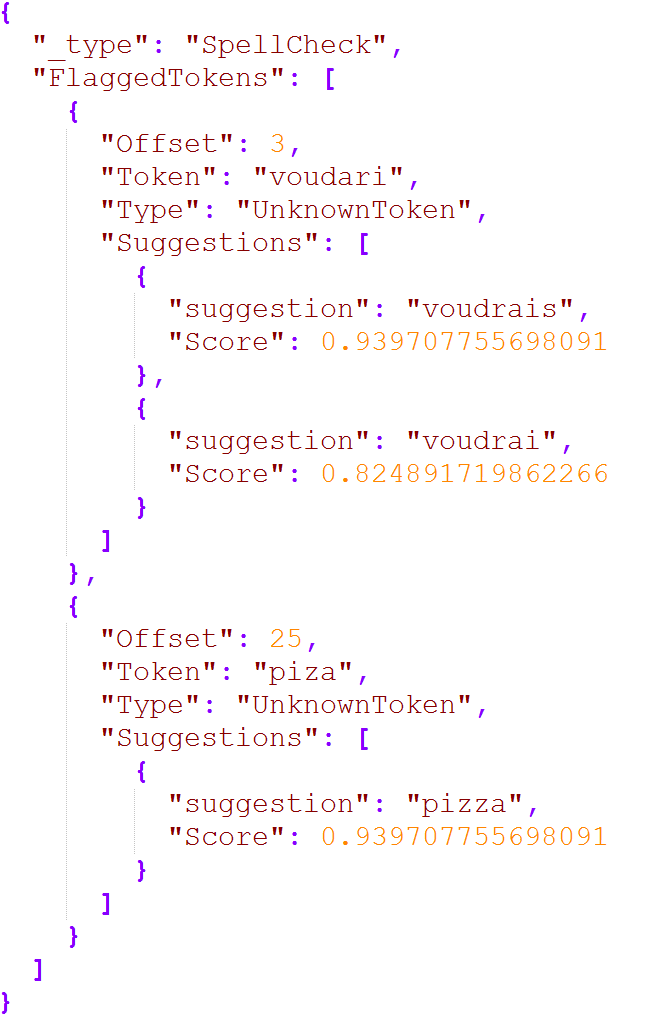
\includegraphics[width = 0.5\textwidth]{JSON.png}
	\caption{Résulat JSON intent order}
	\label{fig:Résulat JSON intent order}
\end{figure}

On peut voir qu’il vérifie voudari qui est mal orthographié et qui correspond plus à voudrais que voudrai. Et que piza est aussi mal orthographié car il manque un ‘z’.
\vspace{1em}


- API Analyse linguistique  segmente une phrase en balise et sert à l’analyse morphosyntaxiques. Cette méthode a été vue dans la partie état de l’art sur le nltk. Pour l’exemple, je prendrai le même mais en anglais  car en français il est pour le moment mal géré.
\vspace{1em}

Exemple : I would like to order pizza :

\begin{figure}[H]
	\centering
		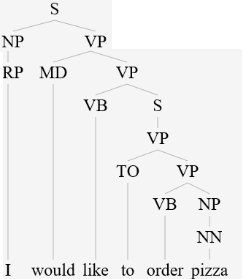
\includegraphics[width = 0.5\textwidth]{analyse.png}
	\caption{Arbre Analyse syntaxique}
	\label{fig:Arbre Analyse syntaxique}
\end{figure}

S : sentence (phrase)
NP : noun phrase (phrase nominal)
VP : verbe phrase (phrase verbale)
RP : particle (particule)
MD : modal
VB : verb (verbe)
TO: to 
NN: noun (nom)


Le lien entre les différents outils repose sur des clés.
\vspace{1em}

Pour notre chatbot programmé avec Microsoft bot framework, il faut l’enregistrer sur https://dev.botframework.com/bots pour obtenir une clé et un mot de passe qui seront ensuite à enregistrer dans le fichier config du projet.  Ces informations seront demandées pour debug avec l’émulateur en localhost.
\vspace{1em}


Bot framework channel emulator :


\begin{figure}[H]
	\centering
		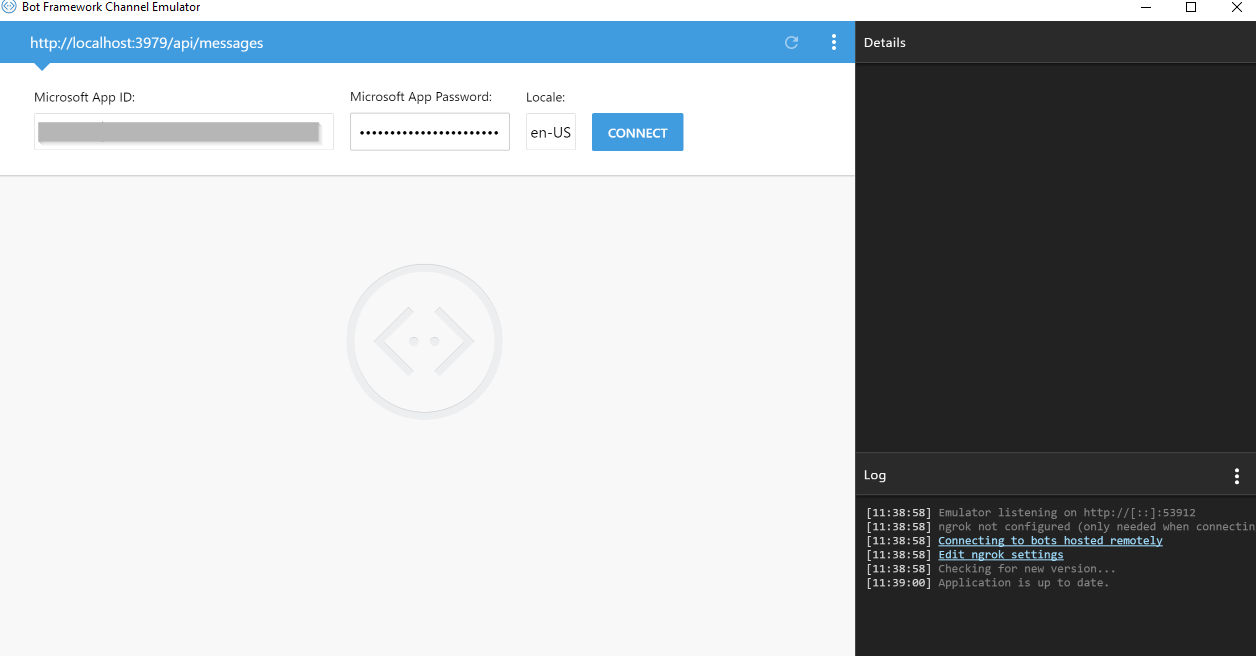
\includegraphics[width = \textwidth]{emulateur.png}
	\caption{Bot framework emulator}
	\label{fig:Bot framework emulator}
\end{figure}

 Pour LUIS, la clé est générée sur « https://www.luis.ai/applications », on construit son modèle et on l’utilise via la clé dans le programme. Ce point sera vu plus en détail dans la partie développement.

\section{Cas concret : incident dans CRM}

Les chatbots exécutent des tâches en répondant à des services ;  lors de mon stage, un besoin était d’en implémenter un pour une entreprise d’assurance fictive nommée Oltiva pour des démonstrations clients avec une interaction entre Dynamics CRM et un chatbot.
\vspace{1em}

Dynamics CRM (Customer Relationship Management) est un logiciel de gestion de la relation clienst pour gérer les ventes, le marketing et les services d’une entreprise. Il permet de suivre l’évolution d’un contact en futur client jusqu’à la vente.
\vspace{1em}

Le scénario est le suivant : 

\begin{figure}[H]
	\centering
		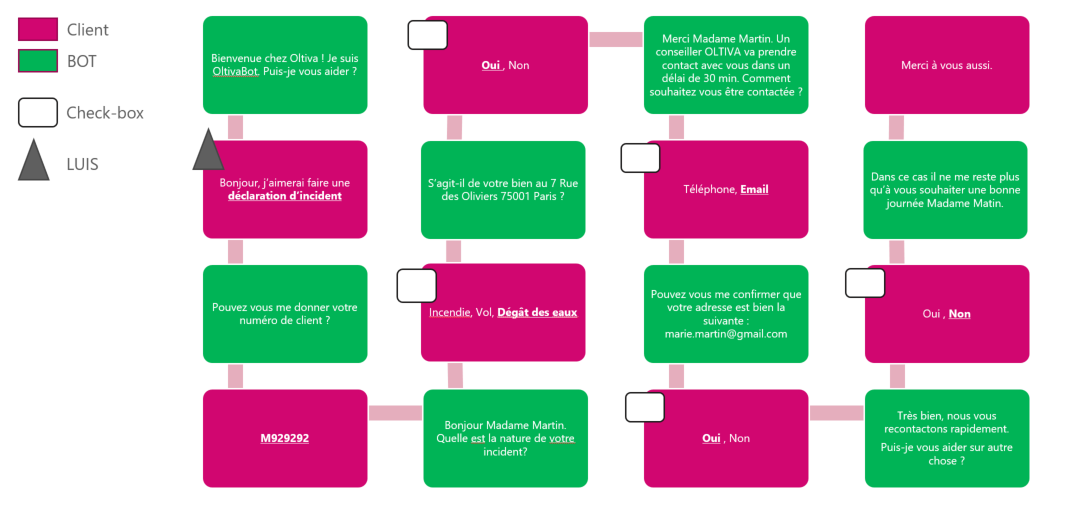
\includegraphics[width = \textwidth]{scenario.png}
	\caption{Scénario incident CRM}
	\label{fig:Scénario incident CRM}
\end{figure}


L’utilisateur veut déclarer un incident, le chatbot demande son identifiant qui est un champ dans CRM pour récupérer toutes les informations du contact. Ensuite le chatbot propose les incidents d’habitation qu’il connait : ce sont les incendies, les vols et les dégâts des eaux. Après avoir choisi, on lui demande si son adresse renseignée dans CRM est la bonne. Ensuite, il lui est proposé la façon dont il veut être contacté par un agent réel (mail ou téléphone) quand son incident sera pris en charge. Il confirme ces informations et s’il n’a pas d’autres questions, alors la conversation est finie.


\section{Développement}

\subsection{Architecture}

Mon architecture est la suivante :


\begin{figure}[H]
	\centering
		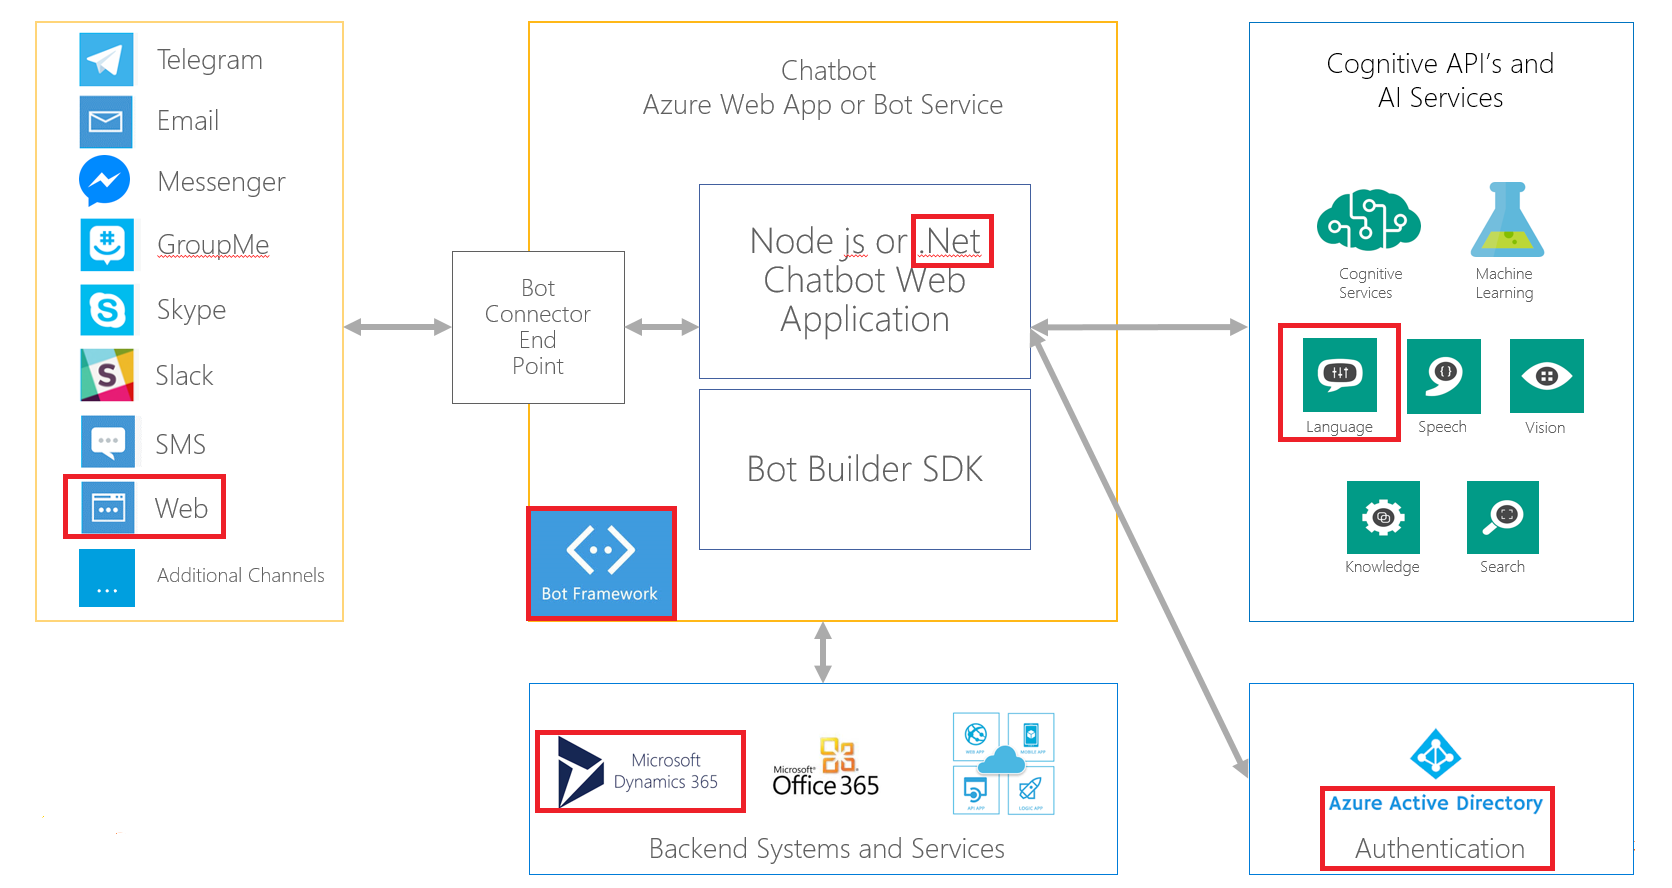
\includegraphics[width = \textwidth]{archi.png}
	\caption{Architecture solution chatbot}
	\label{fig:Architecture solution chatbot}
\end{figure}

On y retrouve le web comme canal qui sera une iFrame présente dans le CRM d’Oltiva. Il sera paramétré sur le site bot framework du bot enregistré.
\vspace{1em}

L’utilisation du Microsoft bot framework qui gère la connexion avec le chatbot est écrite en .NET. On a besoin du sdk, d’une clé et d’un mot de passe (fourni après enregistrement du bot sur le site).
\vspace{1em}

On aura une connexion Dynamics CRM en utilisant le sdk CRM (XRM). Il faut le nom de domaine du CRM et un compte actif (administrateur) avec id et mdp qui seront encryptés.
\vspace{1em}

Il y aura l’utilisation du service azure language (LUIS). On publie sur azure le chatbot pour être ensuite utilisable sur les canaux via Visual Studio. On enregistre notre bot sur LUIS pour obtenir notre modèle et l’utiliser.
\vspace{1em}

Pour revenir au scénario, il est modifié en mettant en avant les interfaces avec CRM :

\begin{figure}[H]
	\centering
		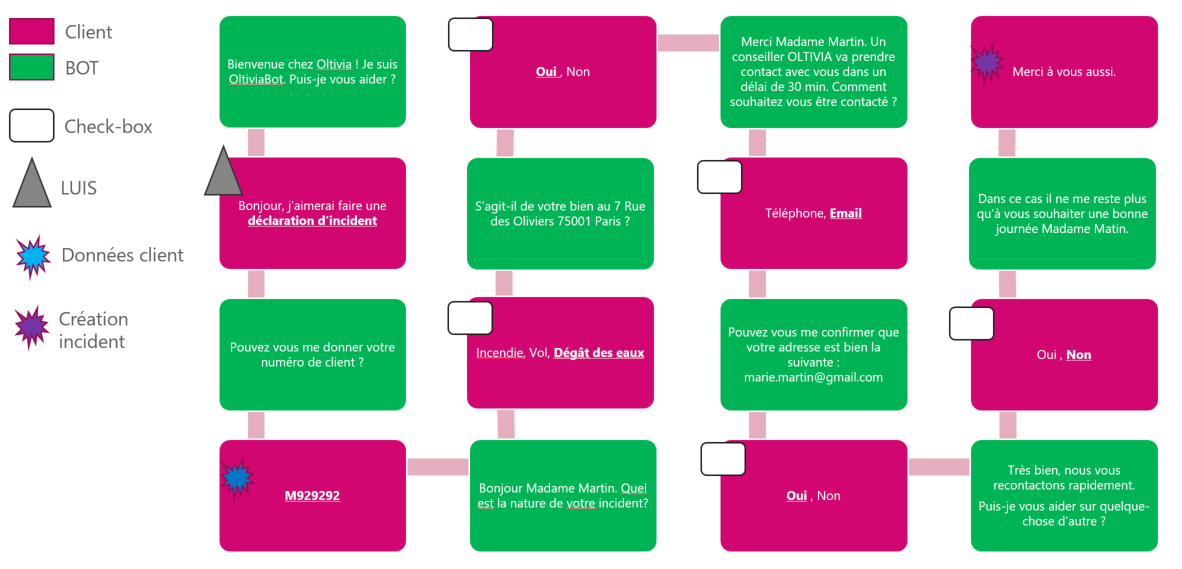
\includegraphics[width = \textwidth]{scenarioInterface.png}
	\caption{Scénario incident CRM avec interfaces}
	\label{fig:Scénario incident CRM avec interfaces}
\end{figure}


LUIS n’intervient qu’au début pour entrer dans un dialogue bien précis avec un certain intent. On aura une connexion avec Dynamics au moment de l’entrée de son identifiant et on la fermera après la conversation pour créer un incident dans CRM avec les informations récupérées.

\subsection{Paramétrage}

Il faut avant tout les intents. On a bonjour, incident pour le scénario et none qui est obligatoire quand aucun autre ne correspond.

\begin{figure}[H]
	\centering
		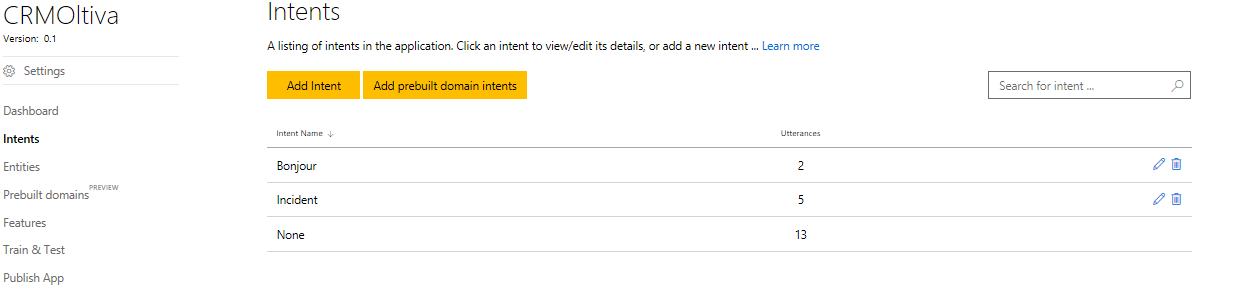
\includegraphics[width = \textwidth]{intent.png}
	\caption{Intents chatbot CRM}
	\label{fig:Intents chatbot CRM}
\end{figure}


On va s’intéresser sur intent avec les utterances suivantes :

\begin{figure}[H]
	\centering
		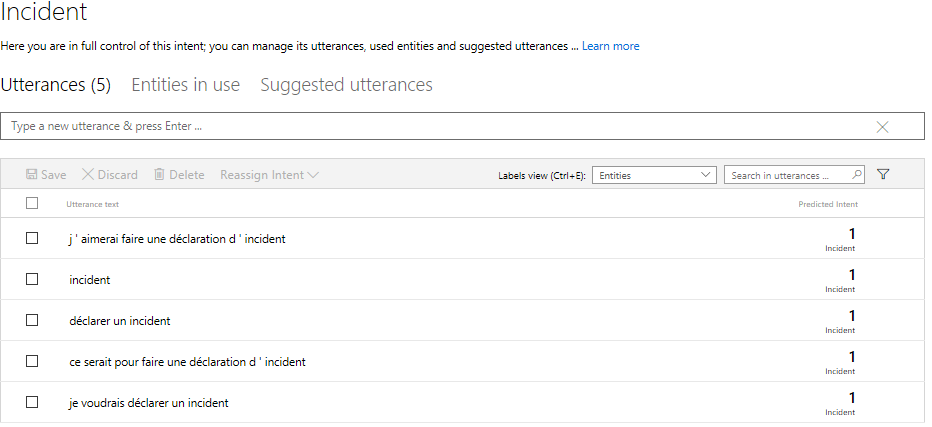
\includegraphics[width = \textwidth]{utterances.png}
	\caption{Utterances intent incident chatbot CRM}
	\label{fig:Utterances intent incident  chatbot CRM}
\end{figure}

On pourrait en rajouter davantage en allant dans l’onglet Suggested utterances qui sont les phrases rentrées par des utilisateurs du chatbot.
\vspace{1em}

Dans le projet, on a un modèle MVC. Le modèle est l’utilisateur qui déclare son incident. Les vues sont les forms flows qui représentent les questions que pose le chatbot dans le scénario. Et le contrôleur gère la messagerie.
\vspace{1em}

Les forms flows sont des dialogues générés automatiquement par le chatbot. L’avantage est d’orienter l’utilisateur tout en générant le ou les questions sur des foms flows appelés précédemment. A la fin, on peut appeler une méthode pour réaliser une action. 
Un exemple pour le premier, c’est de demander l’id utilisateur. Ensuite, on se connecte à CRM et on fait une requête sur l’id puis on instancie notre modèle.
\vspace{1em}

Le contrôleur va appeler une classe qui contient le modèle LUIS pour correspondre avec un l’intent incident. Quand ce sera fait, on aura un enchaînement de méthodes pour représenter le scénario avec un appel successif des différents form flows. Voir Annexe \ref{Code}.
\vspace{1em}

Les forms flows sont modulaires, ils ne dépendent en aucun cas des autres.
\vspace{1em}


\section{Résultat}


Si on teste notre modèle sur la plateforme avec un intent qui n’existe pas mais en lien avec un incident « je voudrais faire une déclaration d’incident », on aurait :

\begin{figure}[H]
	\centering
		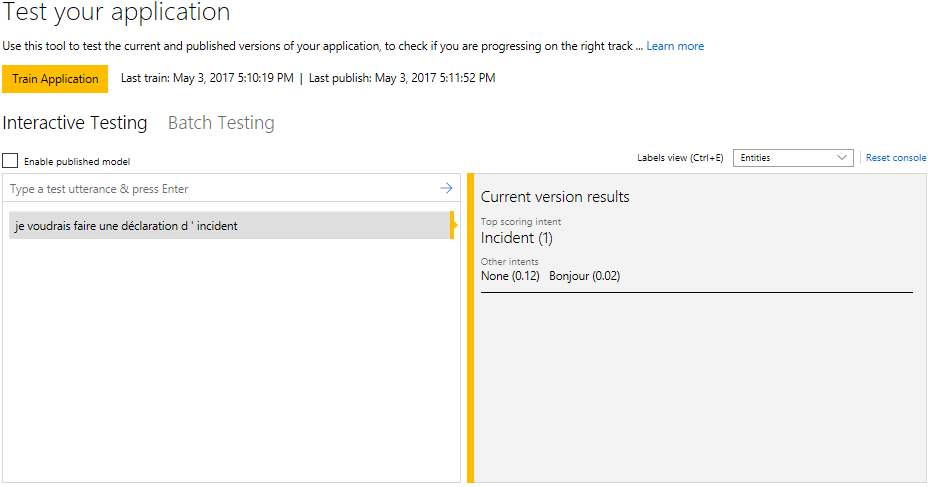
\includegraphics[width = \textwidth]{test1.png}
	\caption{Test intent incident bon}
	\label{fig:Test intent incident bon}
\end{figure}


Cela correspond à une précision de 100\% pour incident, 12\% pour None et 2\% pour Bonjour.
\vspace{1em}

La même phrase avec une faute d’orthographe sur incident :
\vspace{1em}

\begin{figure}[H]
	\centering
		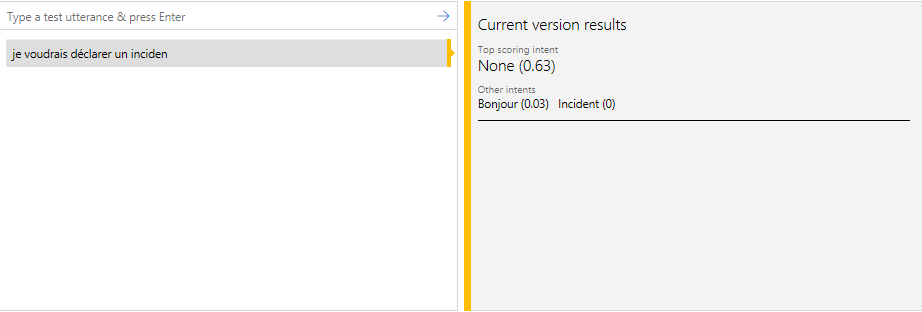
\includegraphics[width = \textwidth]{test2.png}
	\caption{Test intent incident mauvais}
	\label{fig:Test intent incident mauvais}
\end{figure}

Il correspond à None à 63\%, Bonjour à 3\% et Incident à 0\%. Ce problème est résolu soit en entrant cette phrase dans les utterances de l’intent incident soit avec une correction orthographique dans le programme avant l’appel du modèle LUIS.
\vspace{1em}

Le résultat du chatbot dans CRM donne ce résultat :

\begin{figure}[H]
	\centering
		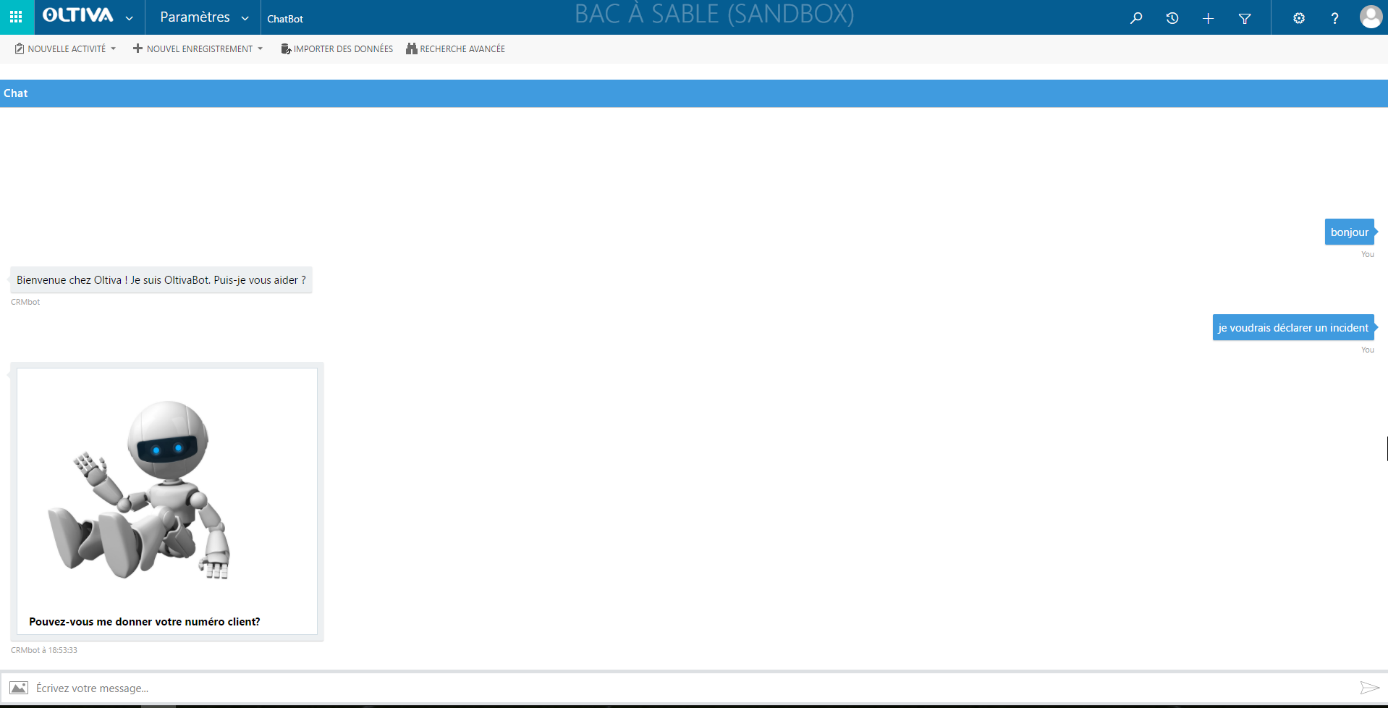
\includegraphics[width = \textwidth]{chat.png}
	\caption{Chatbot CRM}
	\label{fig:Chatbot CRM}
\end{figure}

Vous pouvez retrouver la suite du dialogue dans l’annexe \ref{Dialogue chatbot}.

\section{Discussion}


Notre solution ne comporte que deux intents donc il n’y a pas de gros problème pour commencer une conversation. Avec la compréhension du langage naturel, on aurait pu ajouter des outils d’analyse en place comme la correction orthographique et l’analyse sémantique. Ce choix a été fait car étant une démonstration client, on a peu de risque d’erreur possible lors de la manipulation. Ces outils restent une évolution possible et ils auraient été obligatoires  si le chatbot avait davantage de tâches possibles liées aux incidents par exemple.
\vspace{1em}

Le chatbot est fonctionnel avec un CRM mais on peut imaginer des connexions avec n’importe quel autre service et l’ utiliser sur la plateforme que l’on veut. Il remplit la tâche d’ajouter un incident en remplissant les informations de l’utilisateur pour ensuite être repris par un agent réel. Dans ce cas, le chatbot fait gagner du temps à une entreprise avec un service clientèle tout en étant simple d’utilisation.
\vspace{1em}

Pour un chatbot en domaine fermé, la compréhension du langage nous a permis de paramétrer au mieux notre solution avec notre intent et les utterances qui étaient le NLU. On a fourni des forms flows pour plus de choix et de modularité. Le NLG utilise les infos de CRM qui constituent une base de connaissances pour offrir des dialogues dynamiques. On peut faire du machine learning en ajoutant différents utterances en s’inspirant de que rentrent les utilisateurs.



\section{Limite de la solution}

LUIS n’est utilisé qu’en imput de la solution ;  lorsque l’on rentre dans le dialogue avec les forms flows, c’est à nous de contrôler ensuite les réponses de l’utilisateur étape par étape.
\vspace{1em}

Comme on l’a dit, on est dans un domaine fermé, ce qui limite les problèmes liés au langage naturel car le dialogue est très orienté. S’orienter vers un domaine plus ouvert accroît les risques d’incompréhension avec notre solution actuelle car la complexité est nettement plus grande.
\vspace{1em}

Les intents et les outils externes pour le compléter permettent d’améliorer les performances de compréhension. Le langage naturel est compris mis à part le discours et le sens des phrases qui sont plus dans des chatbots purement conversationnels sans but réel.
\vspace{1em}

Il n’y a pas vraiment de NLG dans la solution car l’utilisateur souhaite déclarer un incident ;  on entre dans l’intent et après il y a un enchaînement de questions que le chatbot pose. Les seuls retours qui sont faits dans ce dialogue ont lieu  lorsque les informations ne sont pas correctes, alors il lui est demandé de les saisir.
